% !TEX root = ../thesis.tex

\chapter{Implementation} \label{implementation}

The primary language used to implement Intertext is Typescript. Typescript is a superset of Javascript that brings it typing support for safety and a better developer experience. Typescript gets transpiled into Javascript during build time, therefor the byproduct is plain Javascript. Sharing the same language between Intertext clients brings a number of advantages, mostly code sharing.

\section{Engine}

Code sharing between Intertext clients has been an important priority while creating the architecture for several reasons. First of all, it is crucial for Intertext clients to behave consistently for some tasks that are common to every Intertext client, such as parsing of IUIDL, rendering of the components, behavioural aspects of the clients, the data structure and so on. These are the cornerstone of Intertext, and they must behave exactly the same across clients. In another words, everything that isn't client-specific needs to be consistent and predictable. This is where Intertext engine comes in play.

Intertext engine implements several aspects of Intertext clients; most notably it parses IUIDL, internally converts it into JSON, and uses the output to render the components. Intertext clients are only concerned with the view layer, but they use the engine as a black box system. The engine also defines the data types of every component, and internal mechanics of the build and rendering process. It exposes the types for Intertext clients built with Typescript to consume. Intertext engine is built as a standalone library, it exposes the main functions and types, and it is designed to be used in several different ways.

At the time of writing, all Intertext clients that are implemented so far were built with Typescript, they simply import and use the engine as a dependency. Their build system picks up the engine and adds it to their final bundle. However this approach is not possible for potential future clients that do not built on a Javascript runtime. To overcome this issue, the engine can be compiled as a Node module, and be deployed to a Node.js server. This gives us the ability to use the engine on any software system that can send or receive HTTP requests. Moreover, with the same logic, the engine can be deployed locally alongside any Intertext client that runs on a platform that can support Node.js runtime. It can then be deployed and served locally, and used to communicate with the local Intertext client using any protocol that is supported by the host platform as long as there exists a data exchange. 

For instance, let's say a car manufacturer wanted to build an Intertext client for their in-car entertainment system using their own components. They could potentially install Node.js on their computer system, or even install a simple raspbery-pi like chip that can run Node.js. Then, they can install the engine as a standalone application in it, and utilize any protocol to build a communication channel between the Intertext client they built on their computer system and the chip. Then, they could serve the IUIDL code either through a network connection (if and when available), or from a locally running server, potentially from the same one the client uses to interact with the engine. 

\section{Layout}

The premise of Intertext is that there will be a unified implementation of UI, in a more or less abstract format, which will then be reified into fully functional front-ends on many different environments. These environments have different requirements and limitations; and an all-in-one solution is needed that will handle all these different requirements and limitations with minimal compromises. One of the aspects that needed consideration was the variation in screen sizes. We had to use a layout system that can be used to build a UI once, and would render properly on various screen sizes.

The obvious solution to this problem was using web technologies, as responsive design is one of the cornerstones of web development. There are many well defined specifications in place to build UI's for different screen sizes. But we cannot directly use web technologies as many of the clients are not browser based. Therefor, we had to use an hybrid approach that can work universally.

\subsection{Layout System}

IUIDL offers a powerful layout system based on the css flexbox specification. It allows developers to build responsive layouts and position UI elements with ease. Intertext web client makes use of the browser implementation of CSS flexbox, whereas for other non-browser based clients, we use Facebook's open source library Yoga \cite{FacebookYoga}. Yoga is a layout engine that implements css flexbox specifications in C++, therefor it can be used on any ecosystem that can execute C++ to calculate the positioning of the UI elements. We currently use Yoga layout engine indirectly on our command-line client, for it was built with a framework that internally uses the Yoga engine.

\begin{figure}[H]
  \centering
  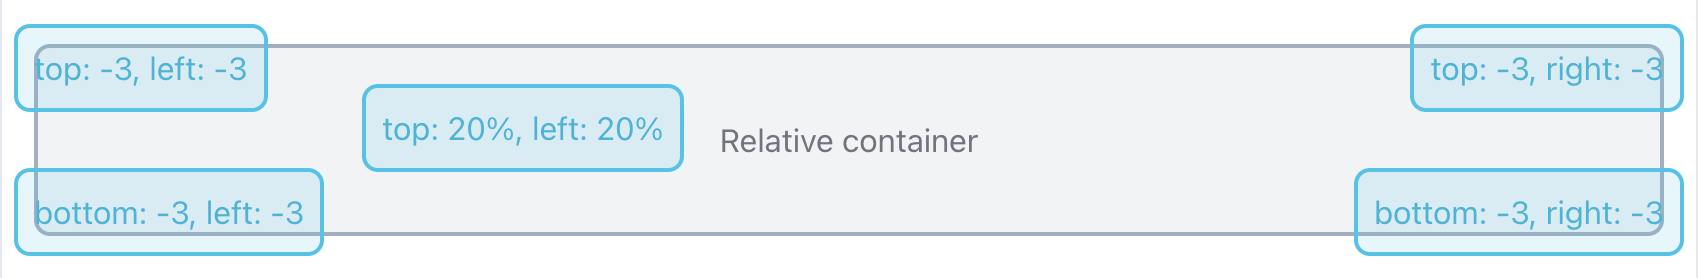
\includegraphics[width=13cm]{thesis/paper/images/absolute.png}
  \caption{Absolute positioning}%
  \label{fig:flexbox_props}%
\end{figure}

Apart from flexbox-based positioning, Intertext layout system also supports absolute positioning. Absolute positioning, as opposed to relative positioning, detaches a component from the flow of the page and positions it relative to its first relatively-positioned parent, having it be floating over everything else, as shown in Figure \ref{fig:absolute_positioning}.

\begin{figure}
  \centering
  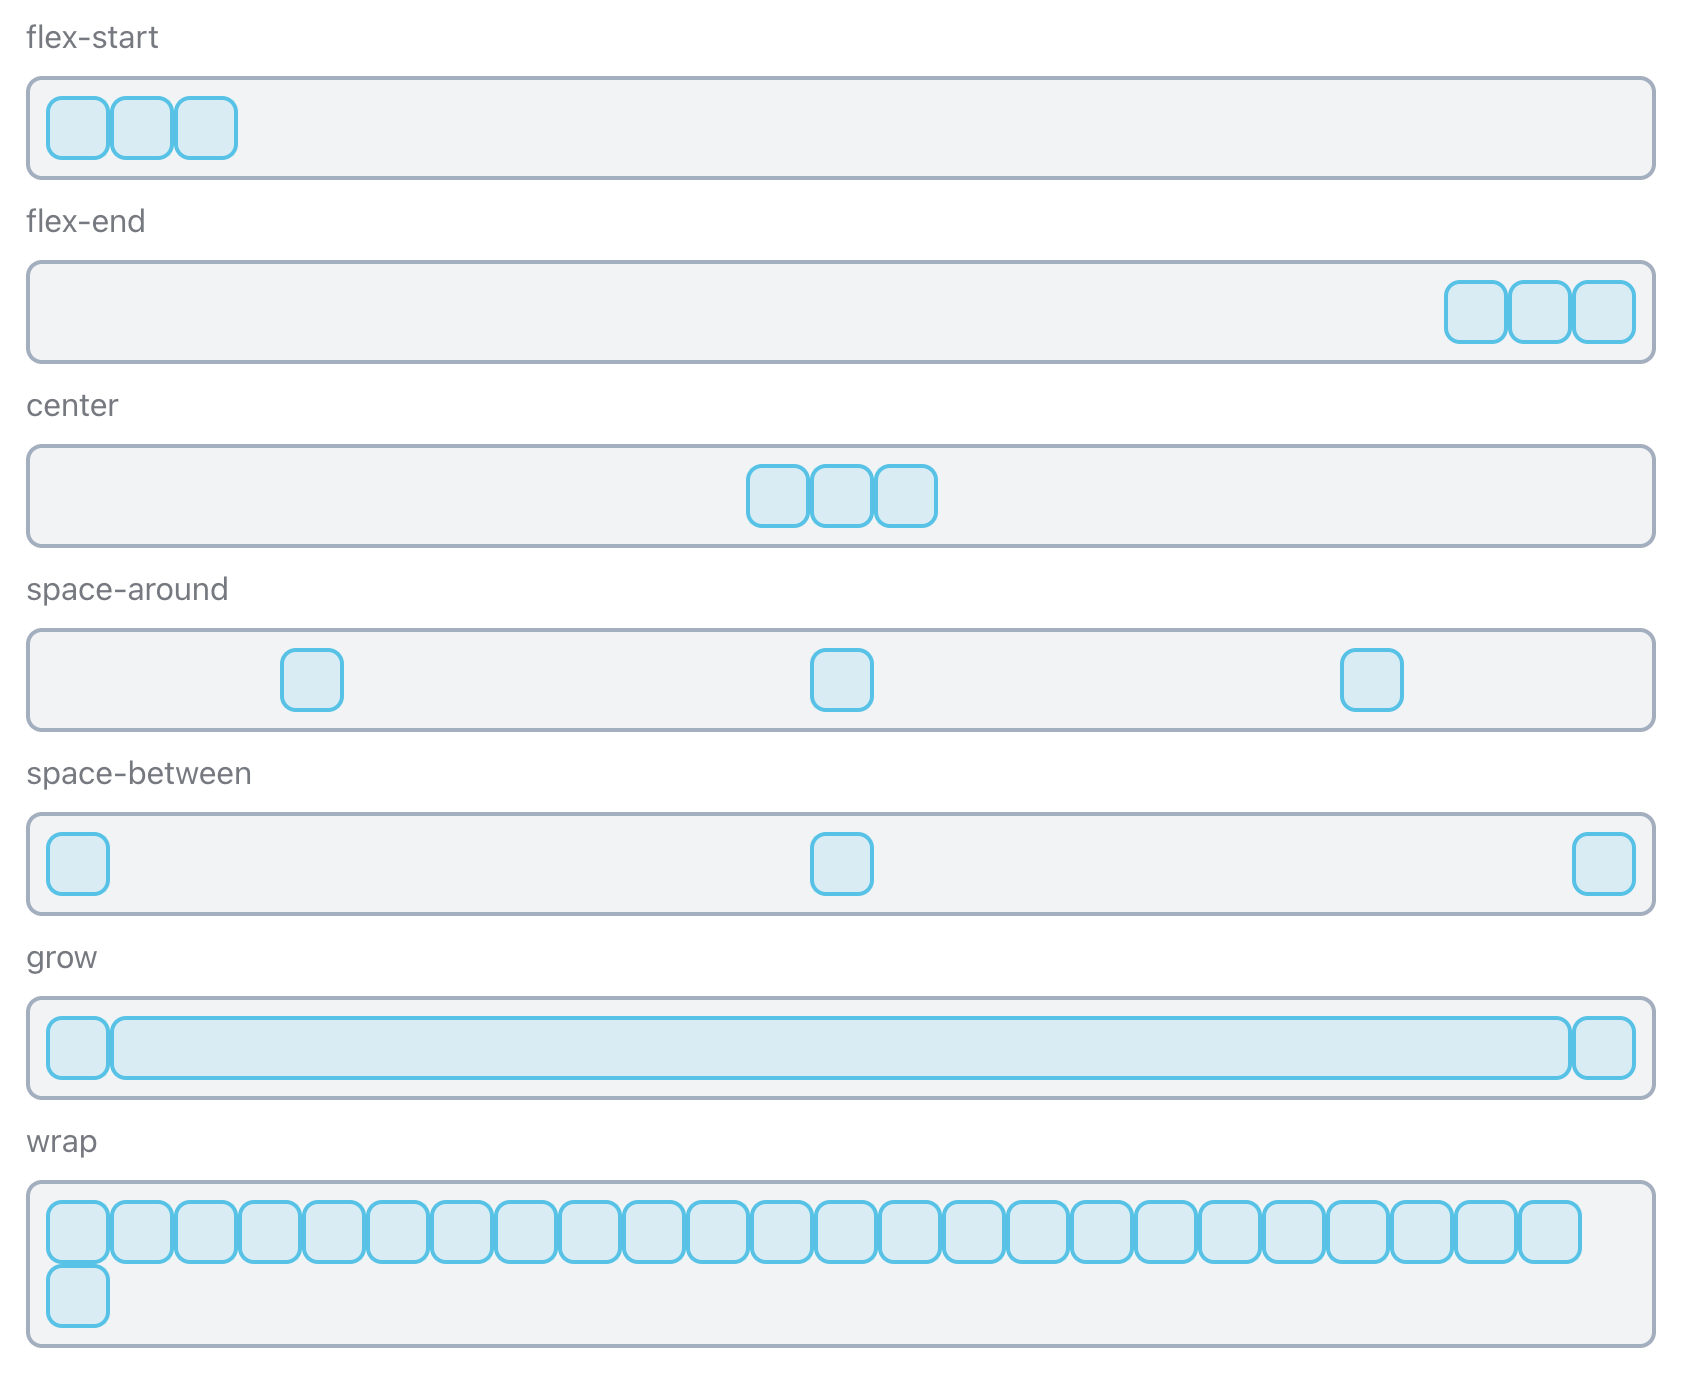
\includegraphics[width=13cm]{thesis/paper/images/responsive.png}
  \caption{Flexbox system}%
  \label{fig:absolute_positioning}%
\end{figure}

One advantage to this approach is that all our clients will render UI elements using the same layout, which will give users a sense of familiarity when switching between the clients. For instance, when a user accustomed to using the web version of Intertext switches to, say the command-line version, they will immediately recognise the layout and be able to navigate without having to adjust. This approach will also allow developers to build responsive layouts to some extent. Given that the same UIDL code will be used to render on multiple clients including ones with narrow and small screens, responsiveness goes a long way. At the time of writing, only flexbox features such as "flex-wrap" can be used for achieving a degree of responsiveness. However we plan to support screen-size aware variants of component properties, even conditional rendering of components based on the screen size. This can be thought of as "media queries" in css terminology. More on this will be on the \nameref{futureWork} section.

\subsection{Unit System}

One of the compromises we had to make for our an all-in-one layout solution was the unit system. We refrained from using definitive units that are specific to one platform, such as pixels. Most platforms use a different measurement system, for instance 1 unit for command-line applications represents a single space; character width for the x-axis and line height for the y-axis.

As a solution, we offer three different types of units; percentages, spaces and sizes. These units can be used for every property that accepts a unit; such as for width, height, margins, paddings and so on. Percentages are universal and can be calculated on any platform that we can get the screen dimensions of. We are able to use it in web environment natively, also the Yoga engine supports percentage values. Spaces are numeric values that starts from 0, increments by 0.5 until 4, by 1 until 12, by 2 until 16, and keeps increasing exponentially until 96. These values are meant to be used for spacing; for paddings, margins, gutter sizes, and other cases where spaces between UI elements needs to be determined. They are mapped to values on different platforms that are reasonable and look approximately same. Finally, we have sizes, which are used for determining the size of UI elements; in properties such as width, height, minWidth/maxWidth, minHeight/maxHeight and so on. While it also makes sense to use percentages for sizes, in cases where sizes should be fixed and not be changing based on the screen size, the size units can be used. Sizes are named values and are mapped to an appropriate value on every platform. They start from 3xs (xsmall) - up to xs, sm (small), md (medium), lg (large), xl (xlarge), 2xl and goes all the way to 8xl.

\subsection{Properties}

\begin{figure}[H]
\begin{minipage}{\linewidth}
\begin{lstlisting}[language=xml]
<block height="24" alignItems="center" justifyContent="center">
  <text>This is centered</text>
</block>
\end{lstlisting}
\end{minipage}
\caption{Layout properties}%
\label{fig:layout_props_example}%
\end{figure}

IUIDL defines some properties that can be used to leverate the layout system to determine sizes, spacing and positioning of UI elements. Figure \ref{fig:layout_props_example} shows an example of how layout properties can be used to center a text in a block. For positioning, \textit{position} prop can be used, which takes \textit{relative} or \textit{absolute}. The default is \textit{relative}. For spacing, supported values are \textit{top}, \textit{bottom}, \textit{left}, \textit{right}, \textit{margin}, \textit{marginTop}, \textit{marginBottom}, \textit{marginLeft}, \textit{marginRight}, \textit{padding}, \textit{paddingTop}, \textit{paddingBottom}, \textit{paddingLeft} and \textit{paddingRight}. As for sizing, accepted values are \textit{width}, \textit{minWidth}, \textit{maxWidth}, \textit{height}, \textit{minHeight} and \textit{maxHeight}. All these values can take all supported unit types. To leverage the flexbox properties, the accepted properties are \textit{alignContent}, \textit{alignItems}, \textit{alignSelf}, \textit{flexDirection}, \textit{flexWrap}, \textit{flexGrow}, \textit{flexShrink}, \textit{flexBasis} and \textit{justifyContent}. Flexbox properties follow the flexbox specification \cite{FlexSpec1} \cite{FlexSpec2}. All layout properties mentioned above are accepted by and can be used with every Intertext component.

\section{Components}

Components are the building block of Intertext applications, they are a set of pre-defined building blocks provided out of the box, which can be assembled to create a functional front-end application. They define the view layer, and they are handled differently on every Intertext client. While the rendering logic and flow of the components are fully driven by engine for consistency, it exposes functions for Intertext clients to register renderers for each component. The renderer function gets called by the engine during the render flow; it receives the props that are the given to the component, the children of the component (if any) that the function is expected to be passing on to the next call level of the recursive rendering flow, and are expected to return the component instance that needs to be rendered, which will later be used to render the UI. Figure \ref{fig:registering_renderer} shows an example snippet of the block renderer being registered to the engine on Intertext web client.

\begin{figure}
\begin{minipage}{\linewidth}
\begin{lstlisting}[language=javascript]
import Engine from "@intertext/engine"
import Block from "../components/core/Block/Block"

const engine = new Engine()

engine.renderer.registerBlockRenderer(({
  index,
  children,
  props,
}) => (
  <Block key={index} {...props}>
    {engine.renderer.render({ branch: children })}
  </Block>
))
\end{lstlisting}
\end{minipage}
\caption{Registering a component renderer}%
\label{fig:registering_renderer}%
\end{figure}

\subsection{Block}

Block component is the most basic and primitive building block of Intertext. It could be thought of as the \textit{div} element of HTML, its main purpose is to enclose components and other blocks. It is primarily a layout component, as it can group and position elements together. Moreover, it can also double as a display component by accepting the \textit{intent} property. When an intent is provided, it renders the block appropriately, thus it can be also used to convey a message. They also accept all layout properties. Figure \ref{fig:intents} shows an example of the block component on the web client, with and without intents.

\subsection{Grid}

Grid is an another layout component that can be used to render its children in grid formation. It accepts \textit{cols} property, which can be used to define how many columns should the grid have, and what the size of the column should be. It accepts numeric values inside curly brackets delaminated with a comma. Number of items in curly brackets represents the number of columns, and each number represents units that the columns should take up, where the total number of units is the sum of the numbers inside curly brackets. For instance, if \textit{cols} value was \textit{[1, 1, 1, 1]}, it would mean that the grid has four columns that are divided equally, where \textit{[1, 3]} would represent two columns with widths being 25\% to 75\%. Grid component also takes a \textit{gap} property to describe the gutter size. It can take any one of the spacing values. Any number of children can be provided to the grid component, without the need to next them in any way, it will automatically position its immediate children based on the given configuration. \ref{fig:grid_xml} shows an example of how grid component can be used, and Figure \ref{fig:grid} shows some render outputs of the grid component for the web client.

\begin{figure}
\begin{minipage}{\linewidth}
\begin{lstlisting}[language=xml]
<grid cols="[2, 3, 1]" gap="2">
  <block intent="info">2</block>
  <block intent="info">3</block>
  <block intent="info">1</block>
  <block intent="info">2</block>
  <block intent="info">3</block>
  <block intent="info">1</block>
</grid>
\end{lstlisting}
\end{minipage}
\caption{How grid component is used}%
\label{fig:grid_xml}%
\end{figure}

\begin{figure}
  \centering
  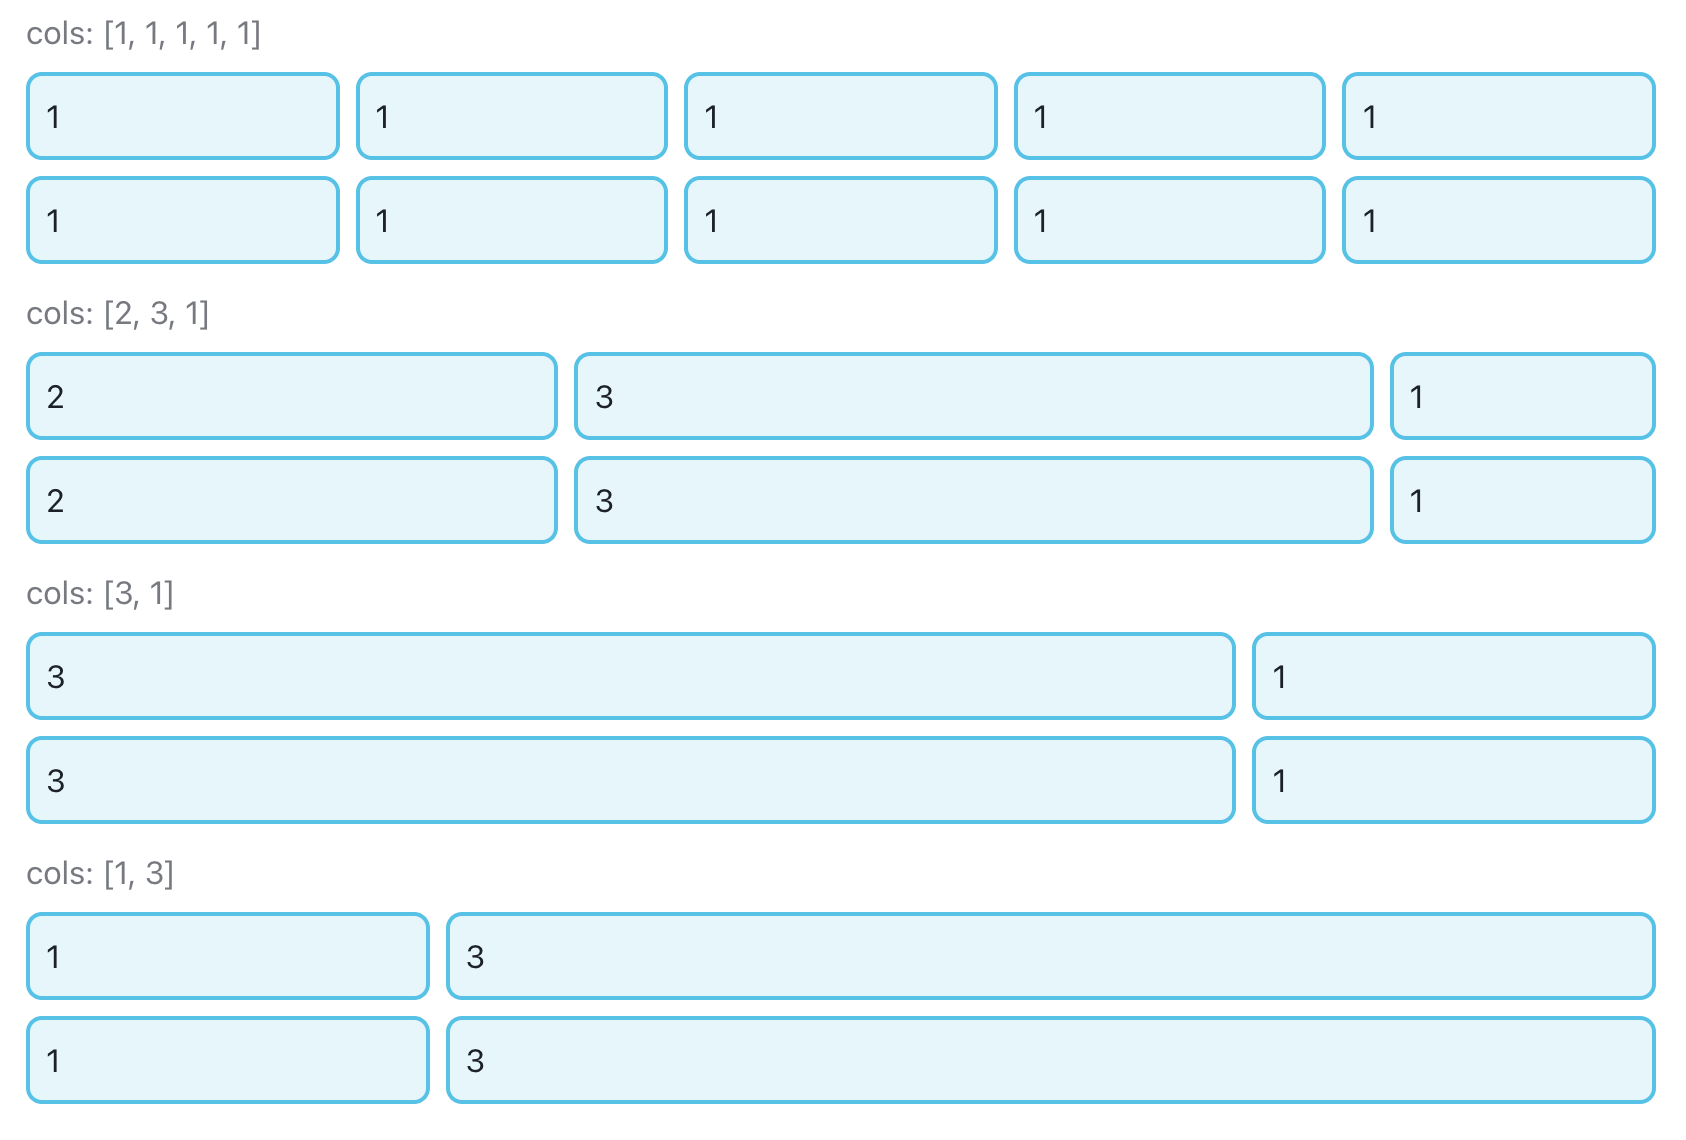
\includegraphics[width=13cm]{thesis/paper/images/grid.png}
  \caption{Grid component}%
  \label{fig:grid}%
\end{figure}

\subsection{Typography}

There are multiple components for typography, most of which are based off of the \textit{text} component. All components for typography stems from the \textit{text} component, but for ease of use, we defined aliases that utilizes the \textit{text} component with a set configuration. The properties that the \textit{text} component accepts are \textit{p}, \textit{h1}, \textit{h2}, \textit{h3}, \textit{b}, \textit{i}, \textit{u}, \textit{block}, \textit{muted}, \textit{code} and \textit{intent}. \textit{p} stands for "paragraph", which is used to define a paragraph block. \textit{h1}, \textit{h2}, \textit{h3} represents headings, and their respective number represents the heading level. The behaviour is similar to HTML. \textit{b}, \textit{i}, \textit{u} are styling options, represents "bold", "italics" and "underlined" respectively. \textit{muted} renders the text with a muted color, useful for descriptions, subtexts or any secondary text that needs to be less attention grabbing. \textit{code} renders the text with a light background and with monospace font family, should be used with codes. 

By default, the \textit{text} component renders inline, meaning, the render output of \textit{<text>1</text><text>2</text>} will appear side by side, as "\textit{12}". However, this behaviour changes for block-level properties; \textit{p}, \textit{h1}, \textit{h2} and \textit{h3}. \textit{text} components that has these properties will take up the full line, and any other text component before or after them will fall into a new line. \textit{block} property is a way to prevent text from rendering inline, without giving it any particular style. Text component also accepts \textit{intent} property, which renders the text with the a color given its intent. Last but not least, text component can accept all layout properties just like any other component. The aliases that can be used in place of \textit{text} are \textit{p}, \textit{h1}, \textit{h2} and \textit{h3} - which will render a \textit{text} component with the respective styles applied. All properties that the text component accepts can be used together to combine styles. For instance, a configuration such as \textit{intent="error", b="true", u="true", h2="true" muted="true"} will result as a red h2 tag, muted, that is bold and underlined.

\subsection{Literals}

Literals are standalone string (or number) values provided to components (other than the \textit{text} component) as children. Figure \ref{fig:text_vs_literal} shows the difference between a literal and a text value. While literals aren't exactly a component themselves, they are nonetheless values that rendering needs to be handled by each client, thus they need their own renderer. The way literals are handled differs from platform to platform, for instance on the web client they can be rendered as is, while on the command line client, they are required to be wrapped within a local Text node.

\begin{figure}
\begin{minipage}{\linewidth}
\begin{lstlisting}[language=xml]
<text>Handled by text renderer</text>
<block><text>Handled by text renderer</text></block>
<block>Handled by literal renderer</block>
\end{lstlisting}
\end{minipage}
\caption{Difference between text and literal nodes}%
\label{fig:text_vs_literal}%
\end{figure}

\subsection{Collapse}

Collapse component can be used to hide long-form content within a collapsible panel that is closed by default, and can be toggled by clicking the handle. It accepts the complex attribute \textit{handle} that takes the contents of the collapse handle. It's children will be rendered inside of the collapse. Collapse components can be nested, in which case each collapse component will operate individually. Figure \ref{fig:collapse_xml} shows how it can be used, and Figure \ref{fig:collapse} shows the render output of a collapse component on the Intertext web client.

\begin{figure}
\begin{minipage}{\linewidth}
\begin{lstlisting}[language=xml]
<collapse>
  <collapse.handle>
    <text>This is the handle</text>
  </collapse.handle>
  <text>This is the content</text>
</collapse>
\end{lstlisting}
\end{minipage}
\caption{How grid component is used}%
\label{fig:collapse_xml}%
\end{figure}

\begin{figure}
  \centering
  
\includegraphics[width=13cm]{thesis/paper/images/collapse_closed.png}
  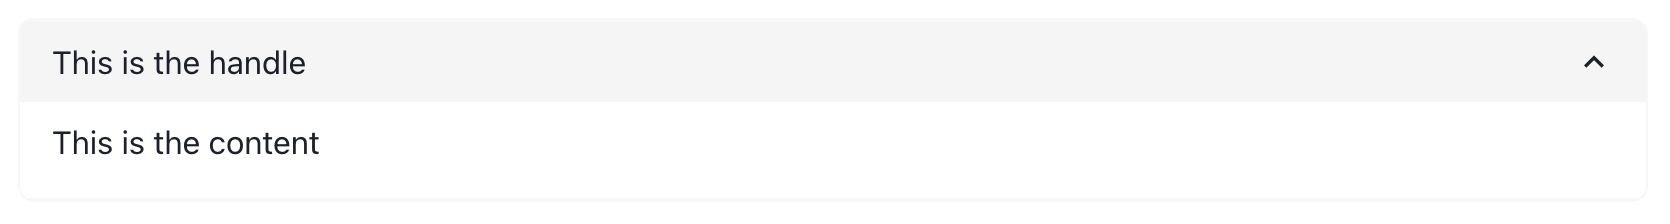
\includegraphics[width=13cm]{thesis/paper/images/collapse_open.png}
  \caption{Collapse component opened and closed state}%
  \label{fig:collapse}%
\end{figure}

\subsection{Button}

Button component is simplest and the most primitive way of triggering commands. It accepts the \textit{onClick} complex attribute, which can accept one or many commands under it.

\subsection{Input}

\section{Commands}

Similar to the components, commands also are registered to the engine. However the registration of the commands are more dynamic compared to the components; while components are static and are immediately available right after the initialization, some commands rely on other artifacts to be available before they are able to be registered. For instance on the web client, the commands related to the client state requires the root component to be mounted, therefor they can only be registered after the mounting occurs. These requirements changes from client to client based on the platform requirements.

\subsection{State}

State command is used to set the state or retrieve read a value from the state. This command is expected to be registered to the engine by each Intertext client based on how the state is handled on the host platform. For instance, for the web client, the client state is controlled by the root component, thus it can only be initialized once the component is initialized and mounted on screen. State command accepts a \textit{key} attribute, which takes the key of the state value to be set. The children of the state command takes the value of the state to be set. Unlike other commands, state command can also be used as a component to display state values on the screen. When the state command is used without providing a value, Intertext engine reads the state value, and interprets it as a literal value, uses the \textit{literalRenderer} to display it on the screen. Figure \ref{fig:how_state_is_set_and_read} shows the syntax of how setting and reading the state works.

\begin{figure}
\begin{minipage}{\linewidth}
\begin{lstlisting}[language=xml]
<!-- set the `name` state value -->
<state key="name">John</state>
\end{lstlisting}
\begin{lstlisting}[language=xml]
<!-- read the `name` state value -->
<!-- renders "Hello, John!" -->
<block>
  <text>Hello, </text>
  <state key="name"></state>
  <text>!</text>
</block>
\end{lstlisting}
\end{minipage}
\caption{How grid component is used}%
\label{fig:how_state_is_set_and_read}%
\end{figure}

\subsection{Alert}

